\subsection{Performance}

\begin{figure*}
  \centering
  \begin{subfigure}[b]{\textwidth}
          \centering
          
\includegraphics[width=0.5\textwidth]{data/legend.pdf}
  \end{subfigure}

  \begin{subfigure}[b]{0.33\textwidth}
      \centering
      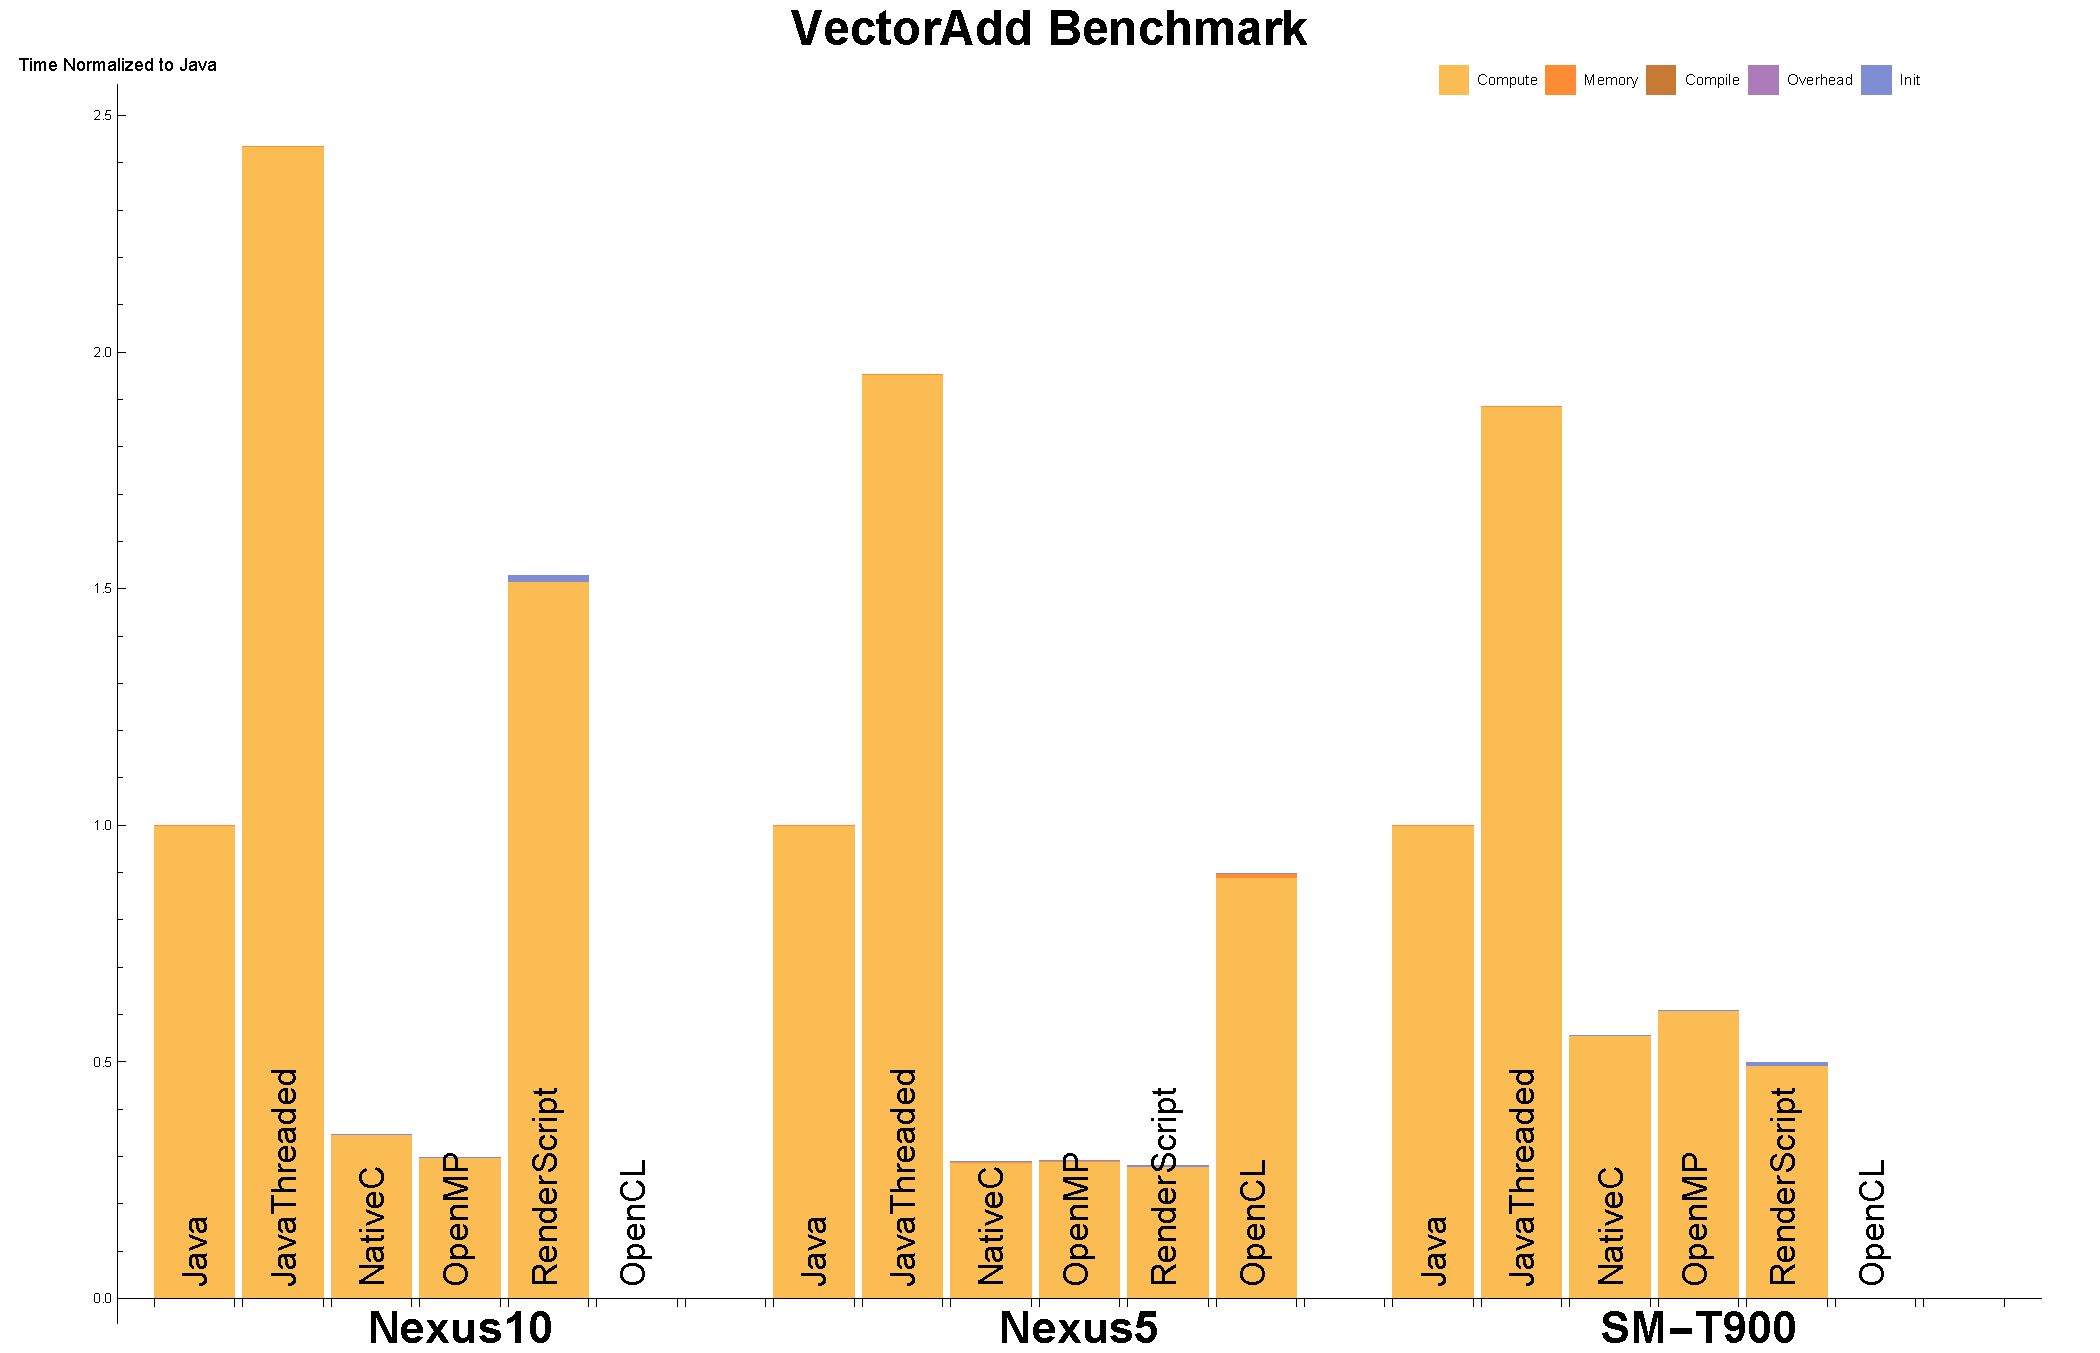
\includegraphics[width=0.9\textwidth]{data/VectorAdd_onecompute_time.pdf}
      \caption{VectorAdd}
  \end{subfigure}
  \begin{subfigure}[b]{0.33\textwidth}
      \centering
      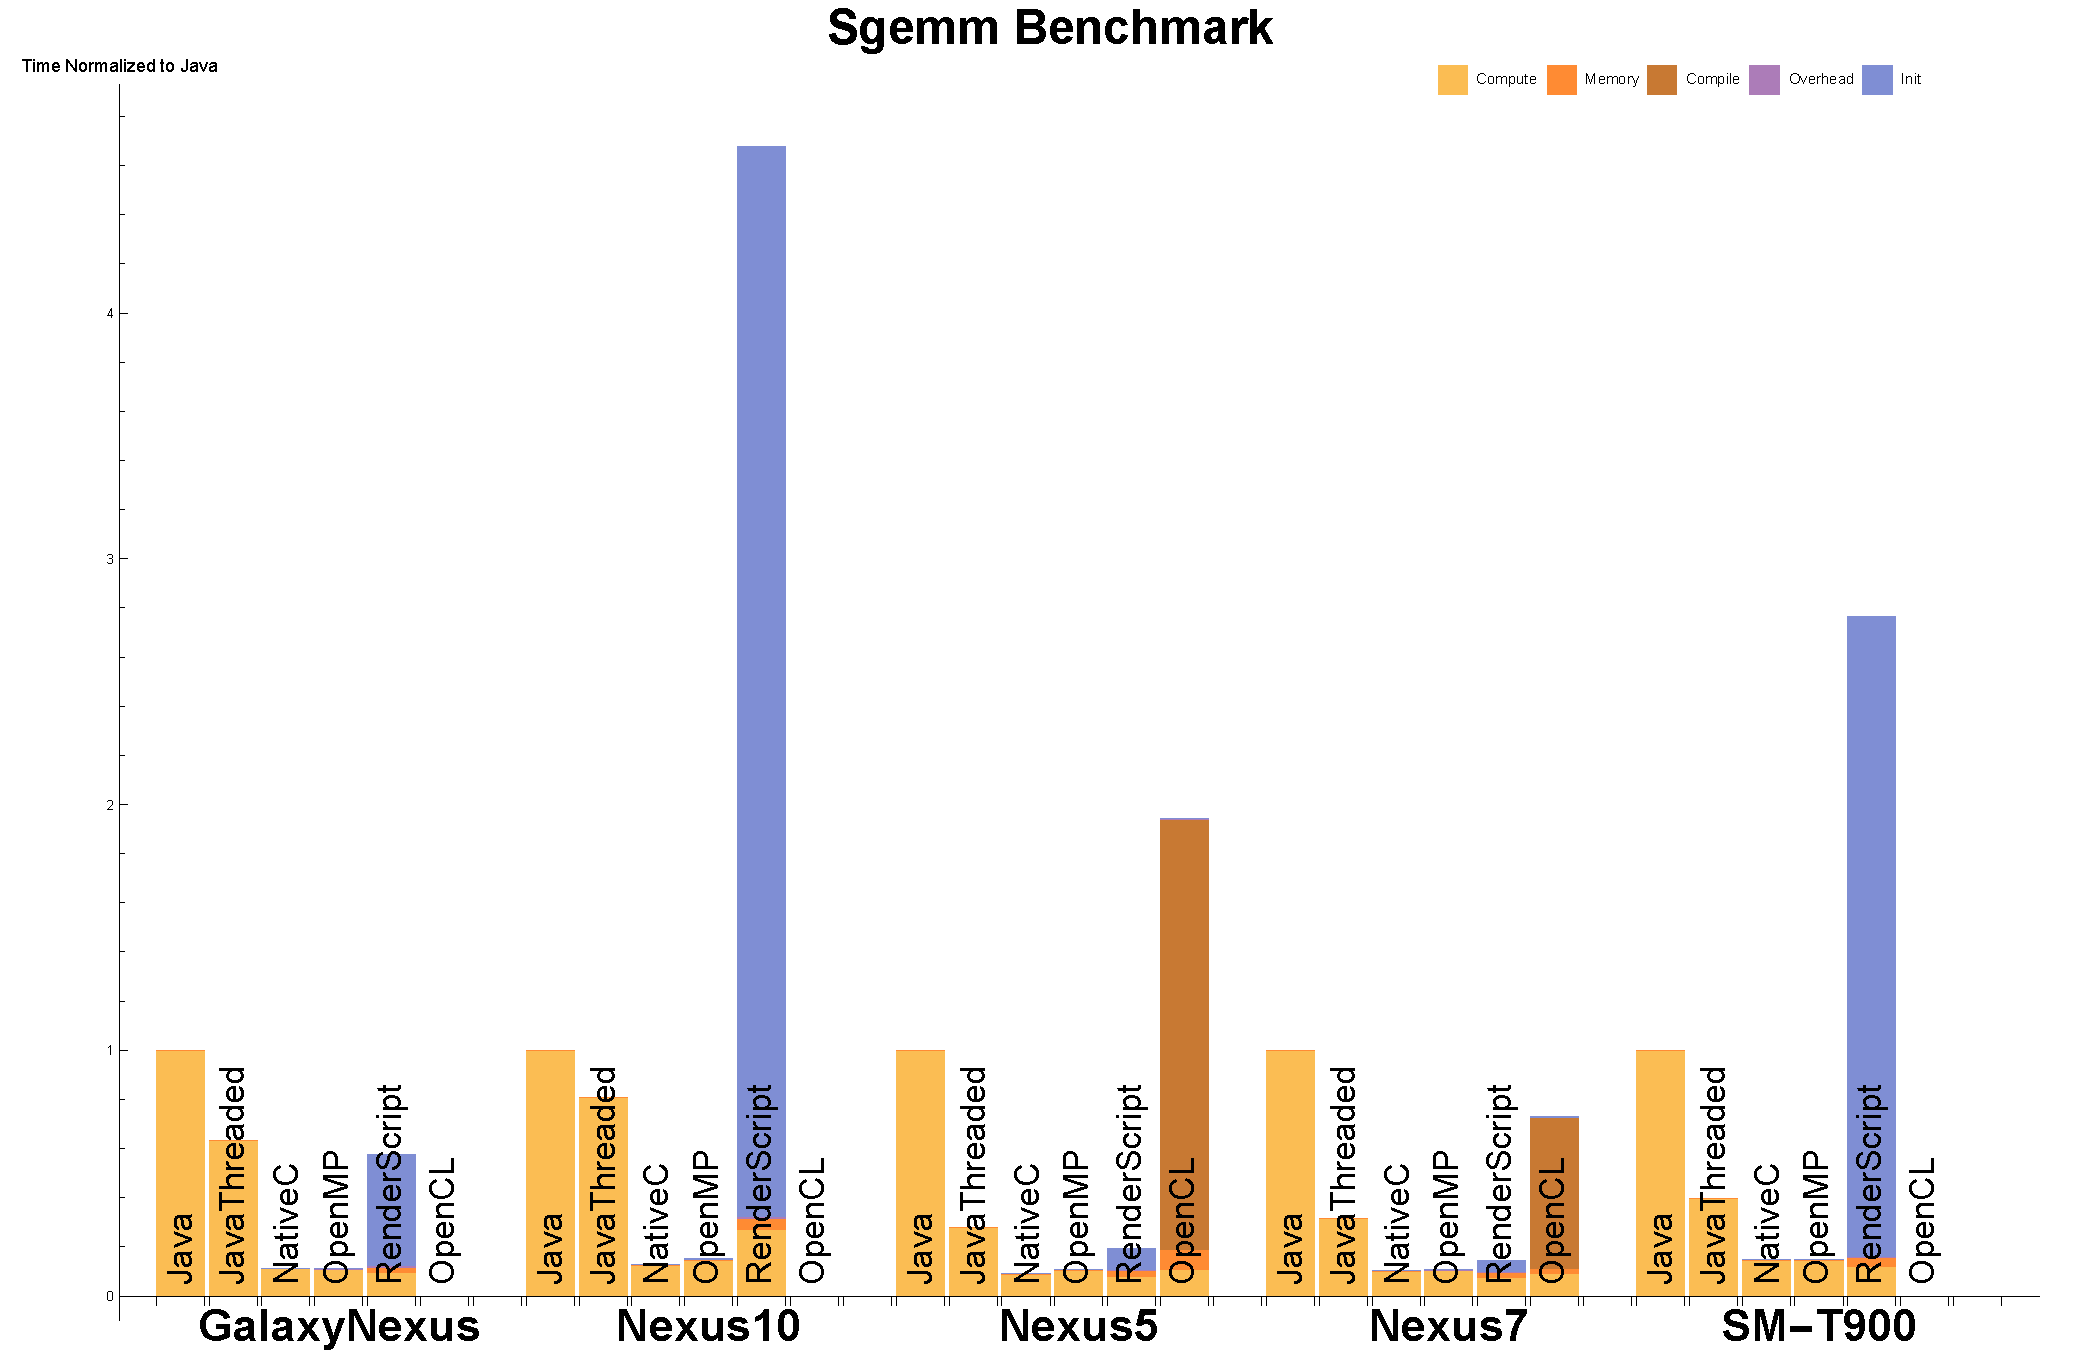
\includegraphics[width=0.9\textwidth]{data/Sgemm_onecompute_time.pdf}
      \caption{Sgemm}
  \end{subfigure}
  \begin{subfigure}[b]{0.33\textwidth}
      \centering
      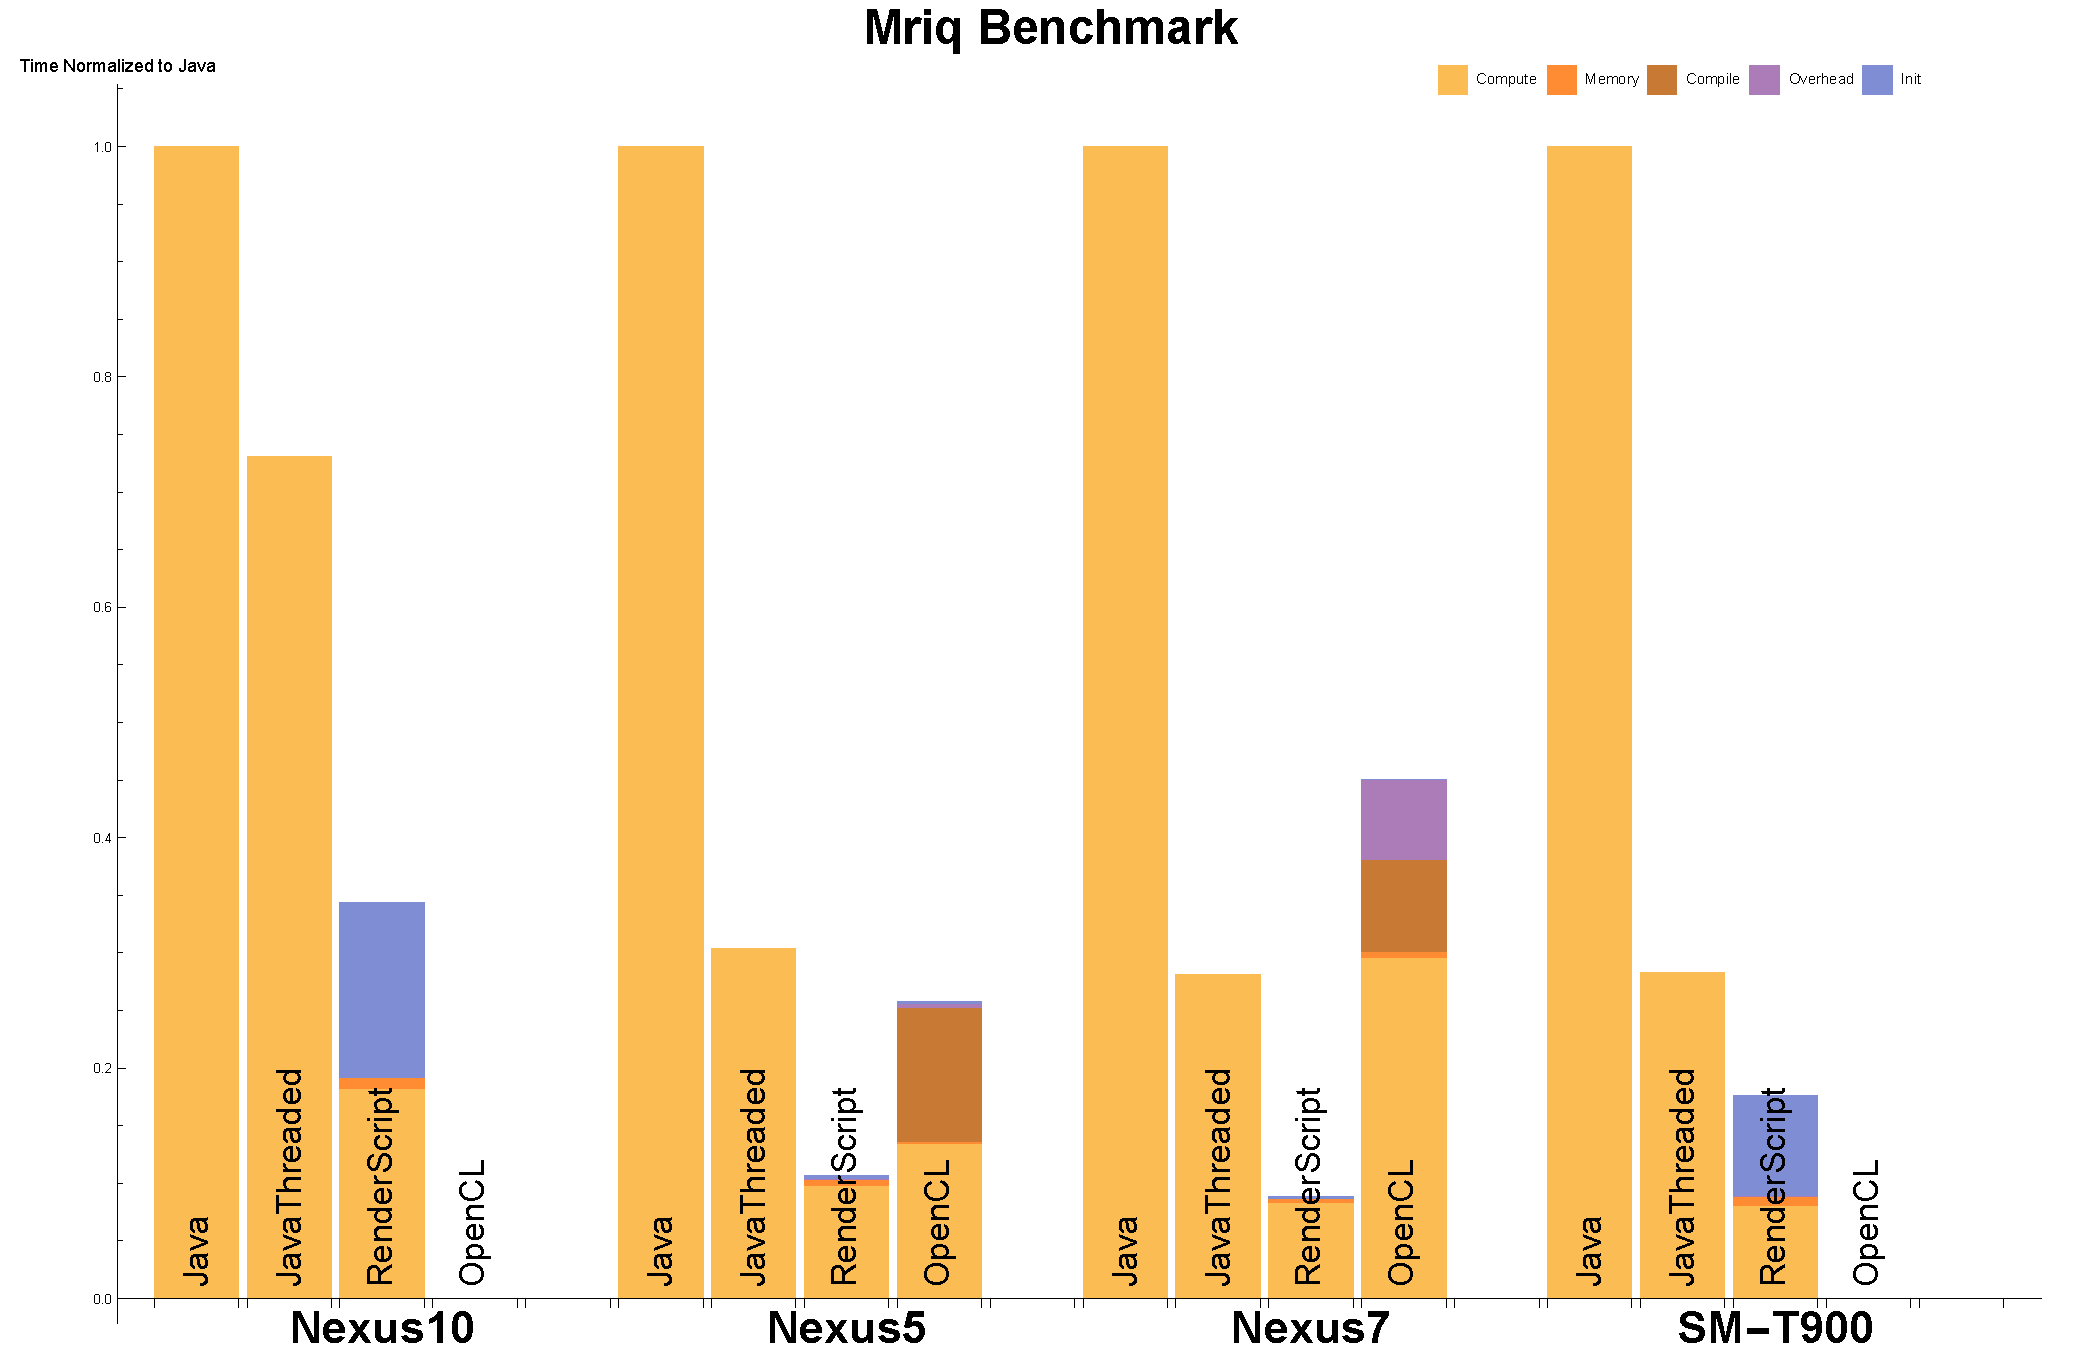
\includegraphics[width=0.9\textwidth]{data/Mriq_onecompute_time.pdf}
      \caption{MRIQ}
  \end{subfigure}

  \begin{subfigure}[b]{0.33\textwidth}
      \centering
      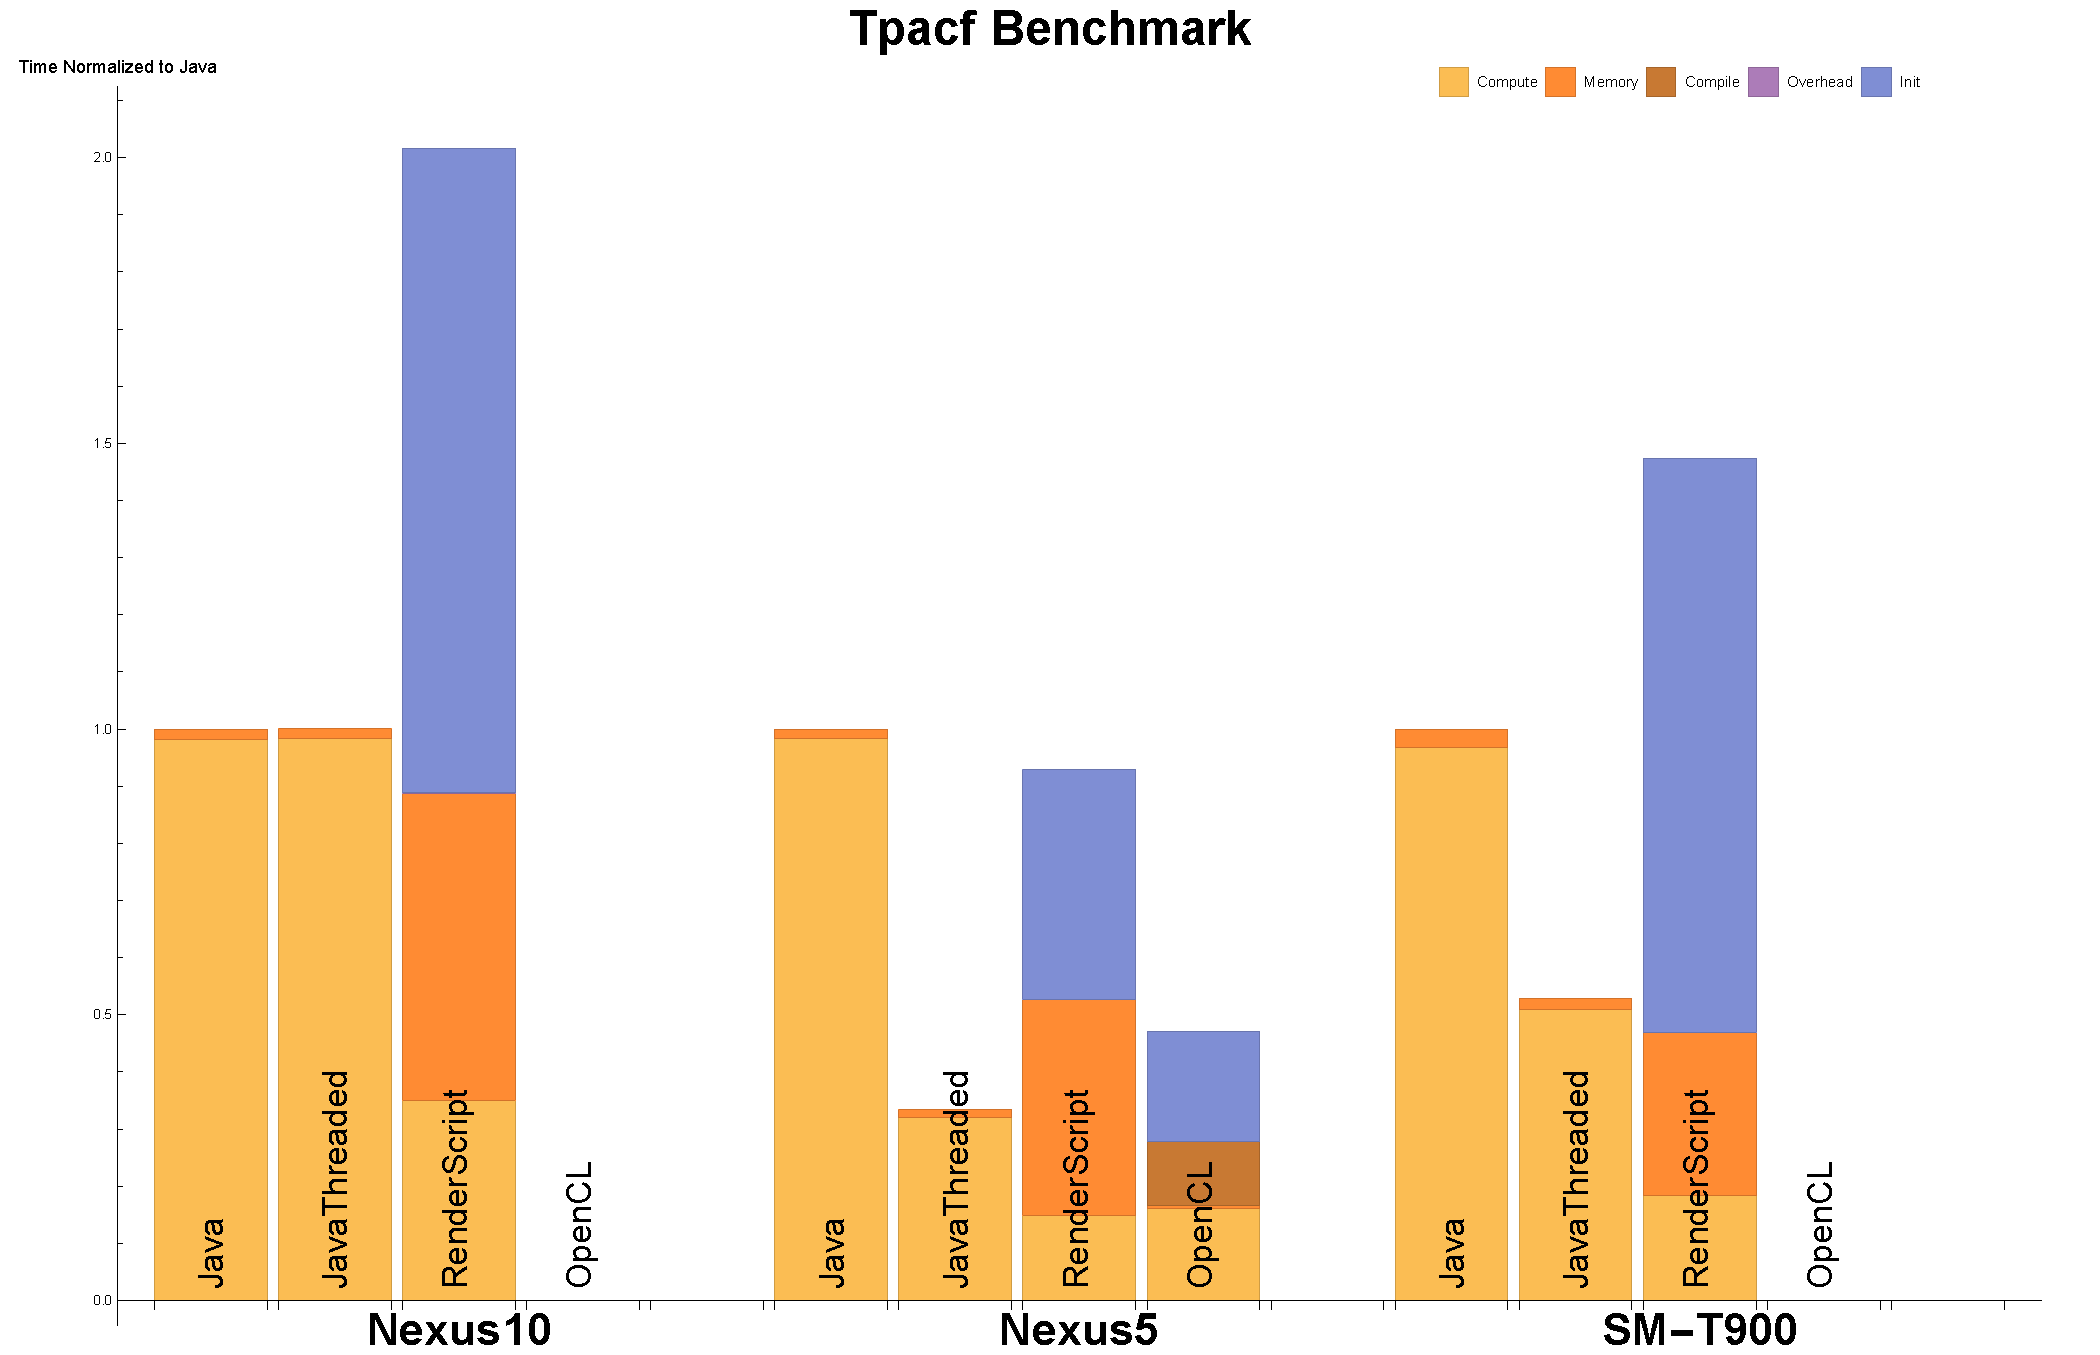
\includegraphics[width=0.9\textwidth]{data/Tpacf_onecompute_time.pdf}
      \caption{TPACF}
  \end{subfigure}
  \begin{subfigure}[b]{0.33\textwidth}
      \centering
      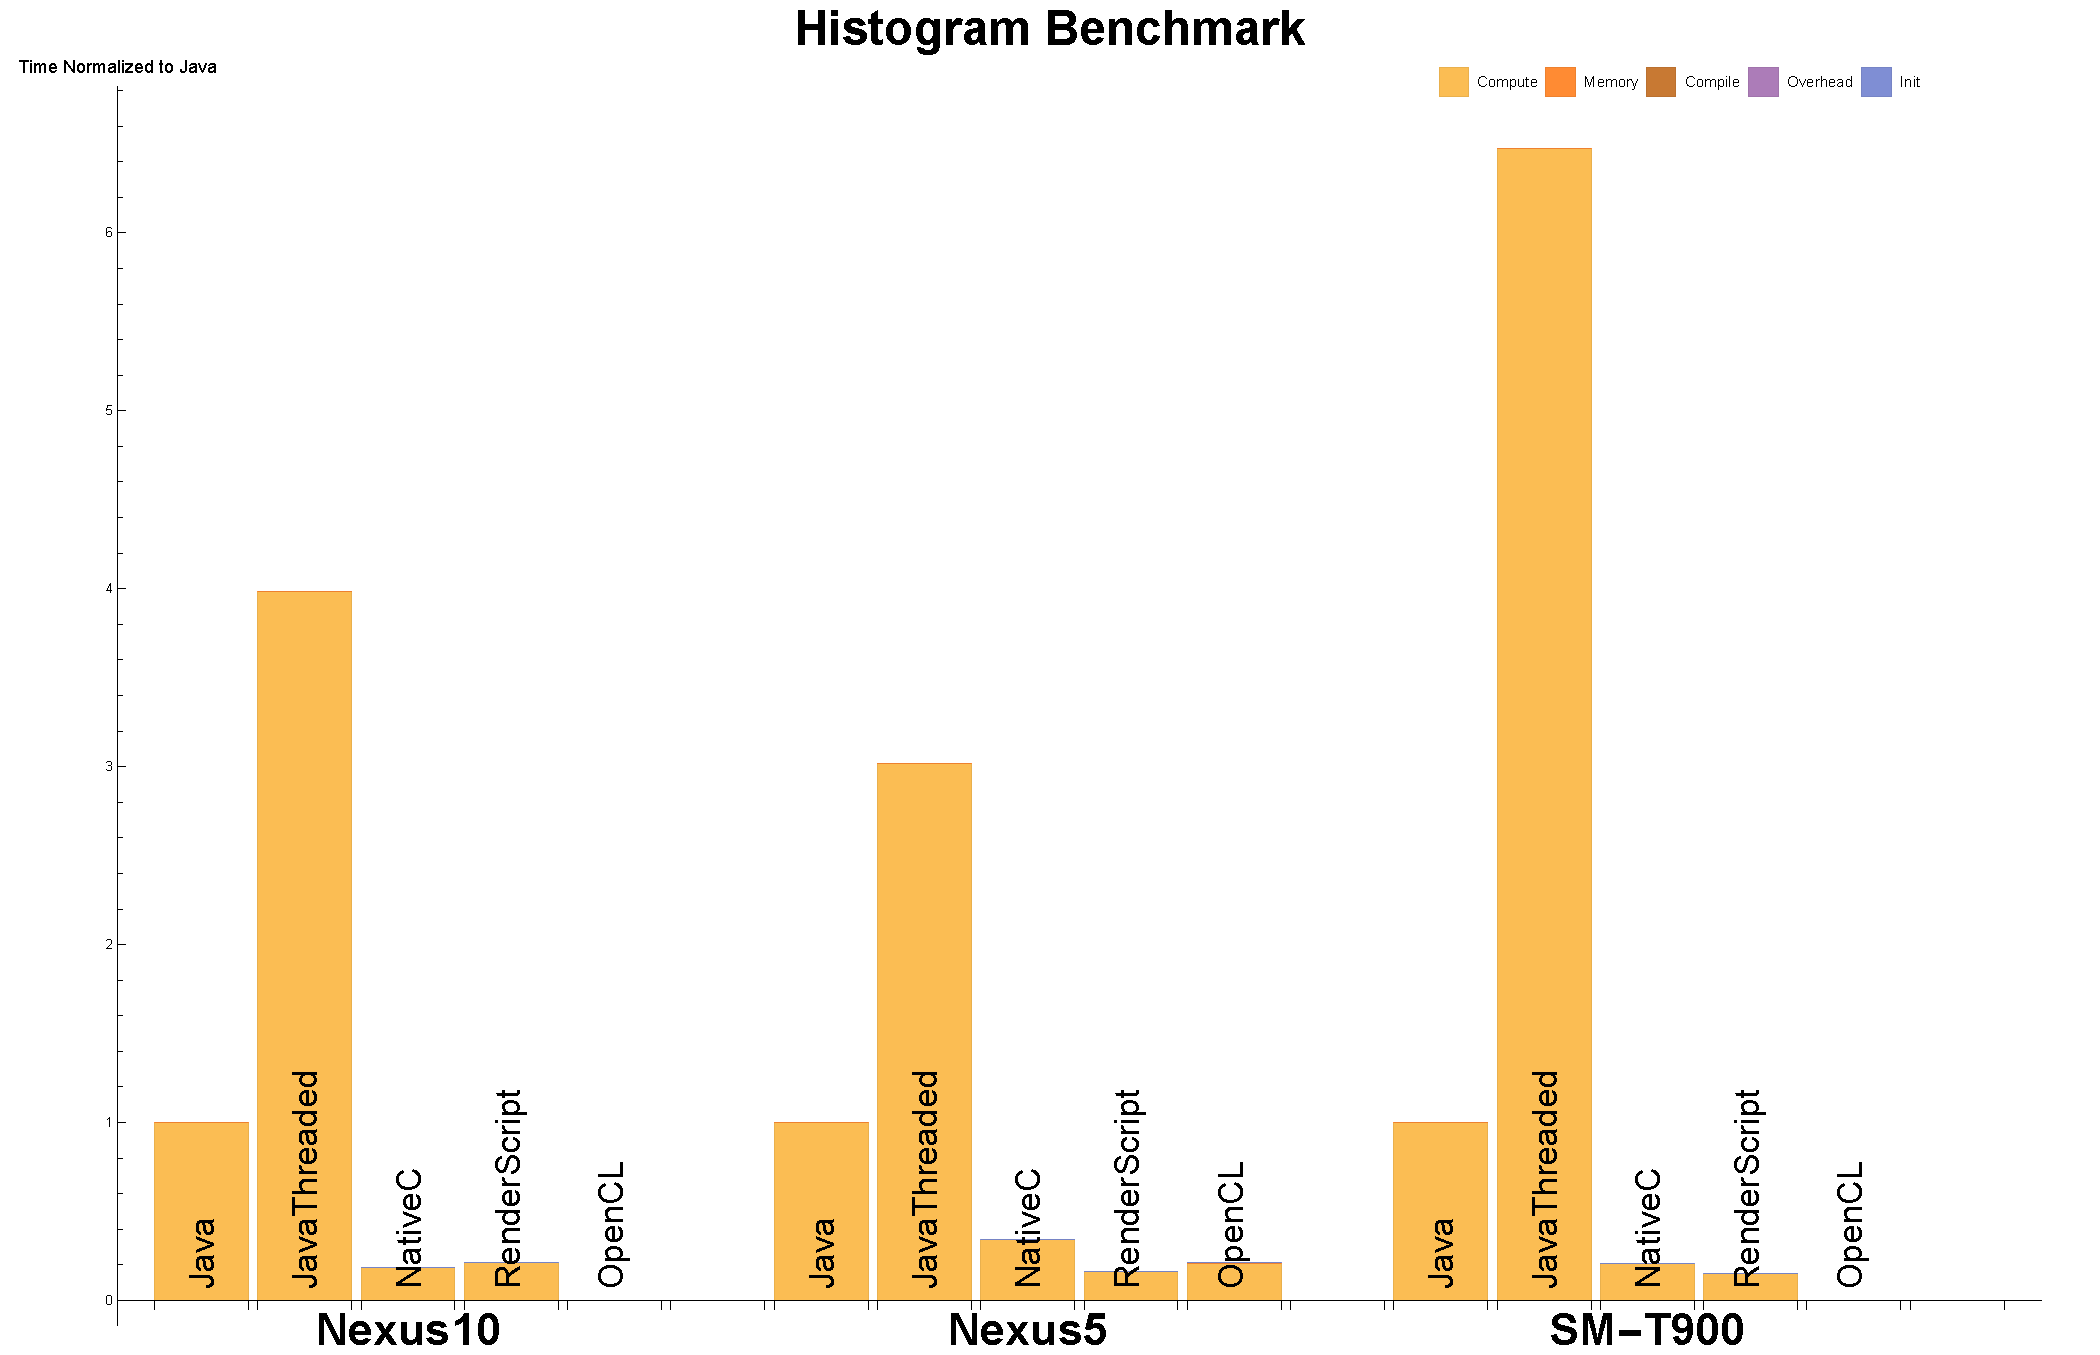
\includegraphics[width=0.9\textwidth]{data/Histogram_onecompute_time.pdf}
      \caption{Histogram}
  \end{subfigure}
  \begin{subfigure}[b]{0.33\textwidth}
      \centering
      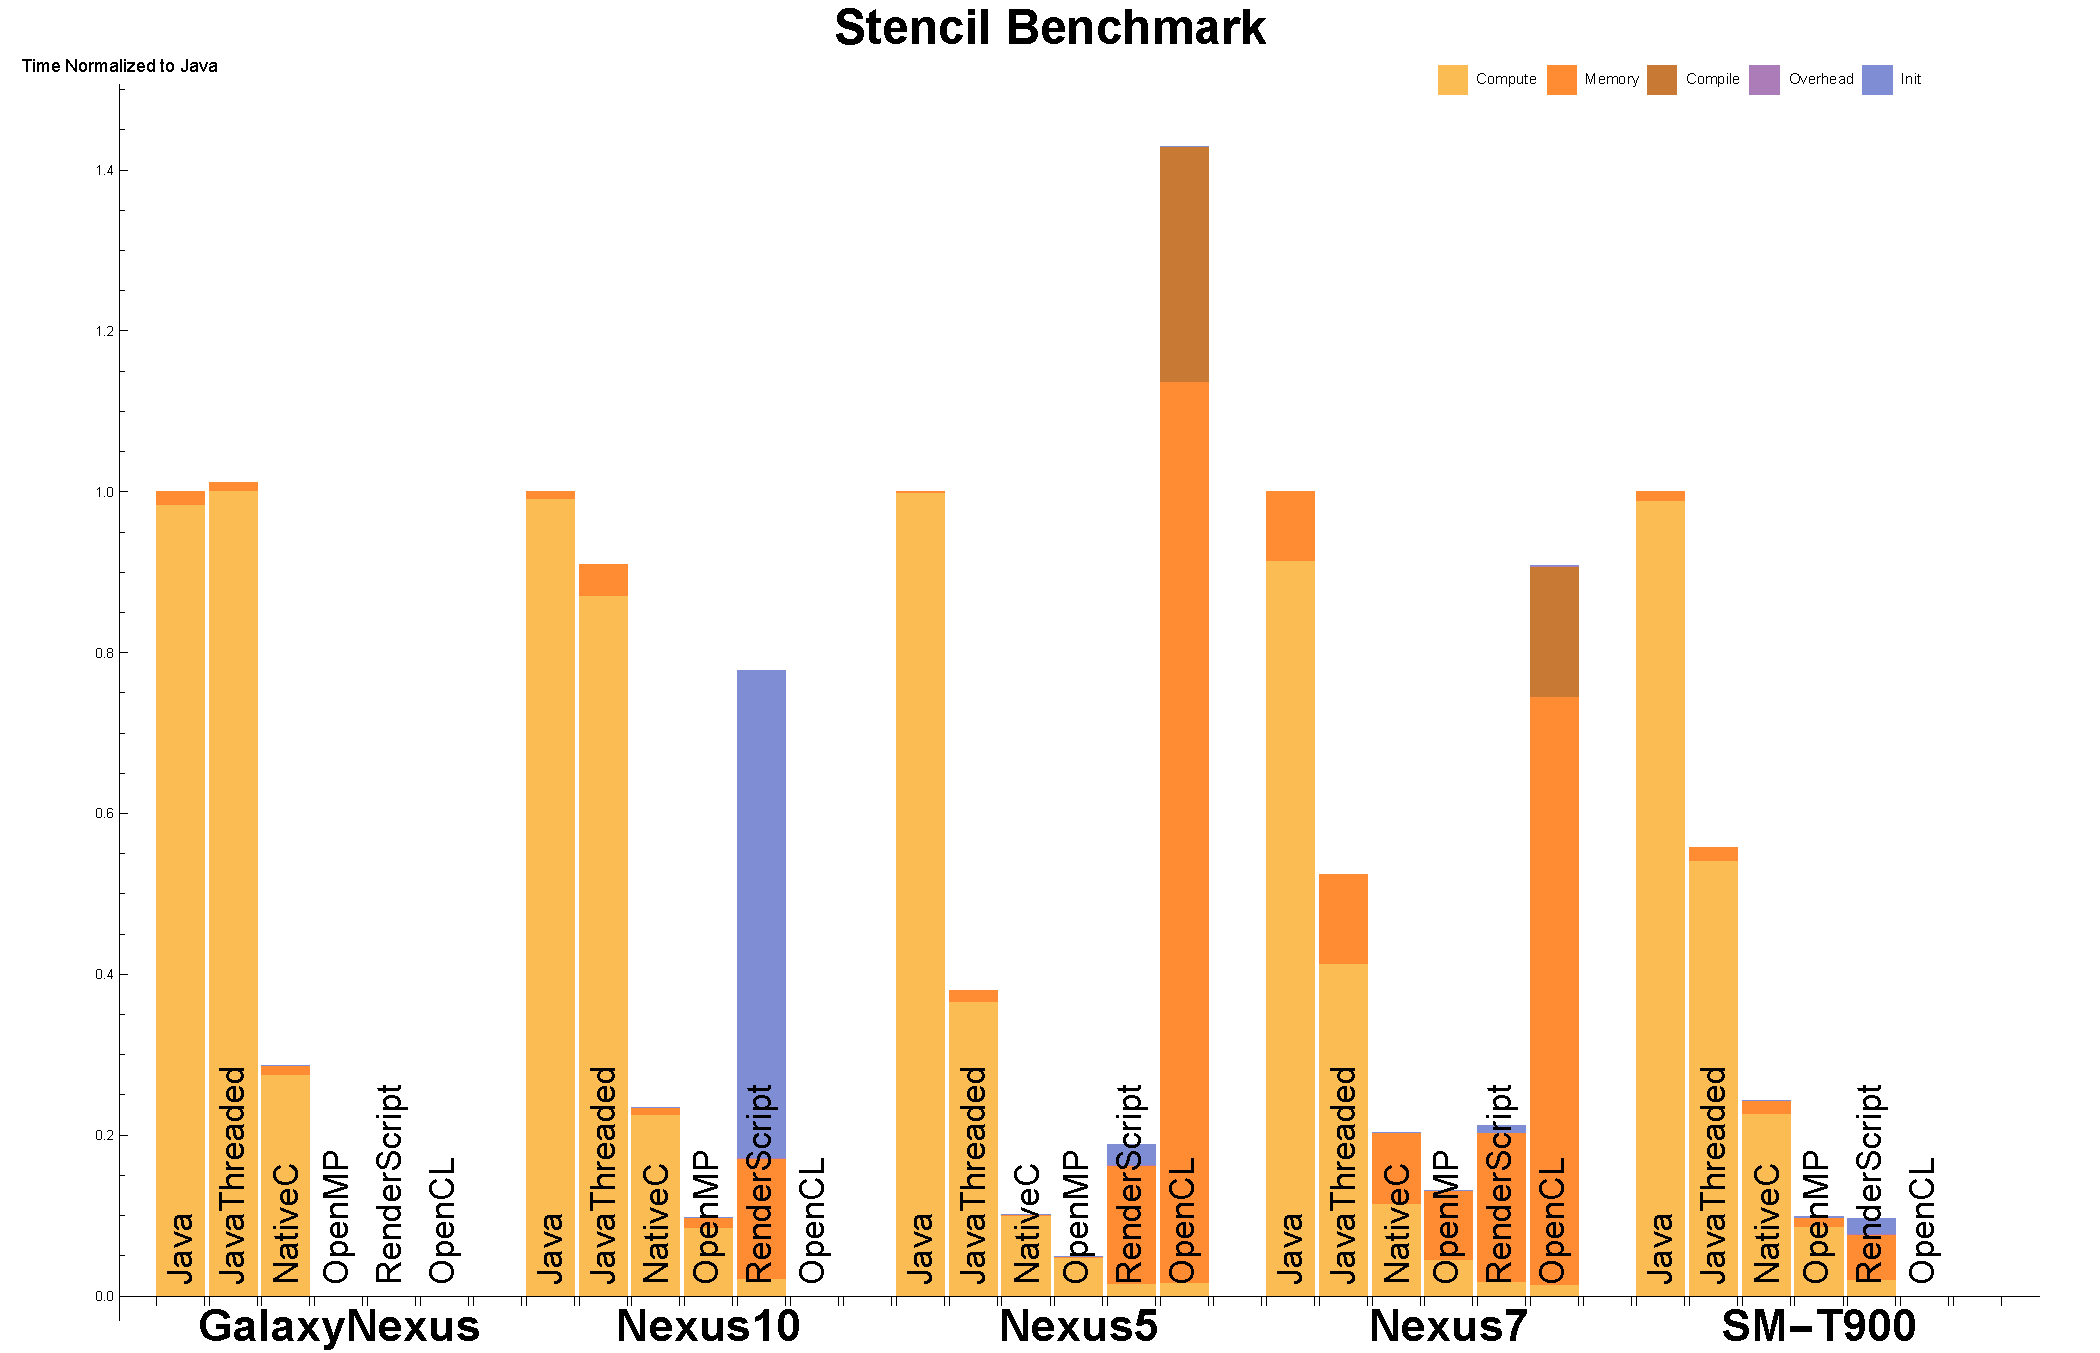
\includegraphics[width=0.9\textwidth]{data/Stencil_onecompute_time.pdf}
      \caption{Stencil}
  \end{subfigure}
  \caption{Runtime across devices where kernel is executed once. The runtime is normalized to the Java execution time (lower is better). J : Java, JT : JavaThreaded, C : Native C, OMP: OpenMP, OCL : OpenCL, and RS : RenderScript.}
  \label{fig:perfOne}
\end{figure*}

\begin{figure*}

  \centering
  \begin{subfigure}[b]{\textwidth}
          \centering
          
\includegraphics[width=0.5\textwidth]{data/legend.pdf}
  \end{subfigure}

  \begin{subfigure}[b]{0.33\textwidth}
      \centering
      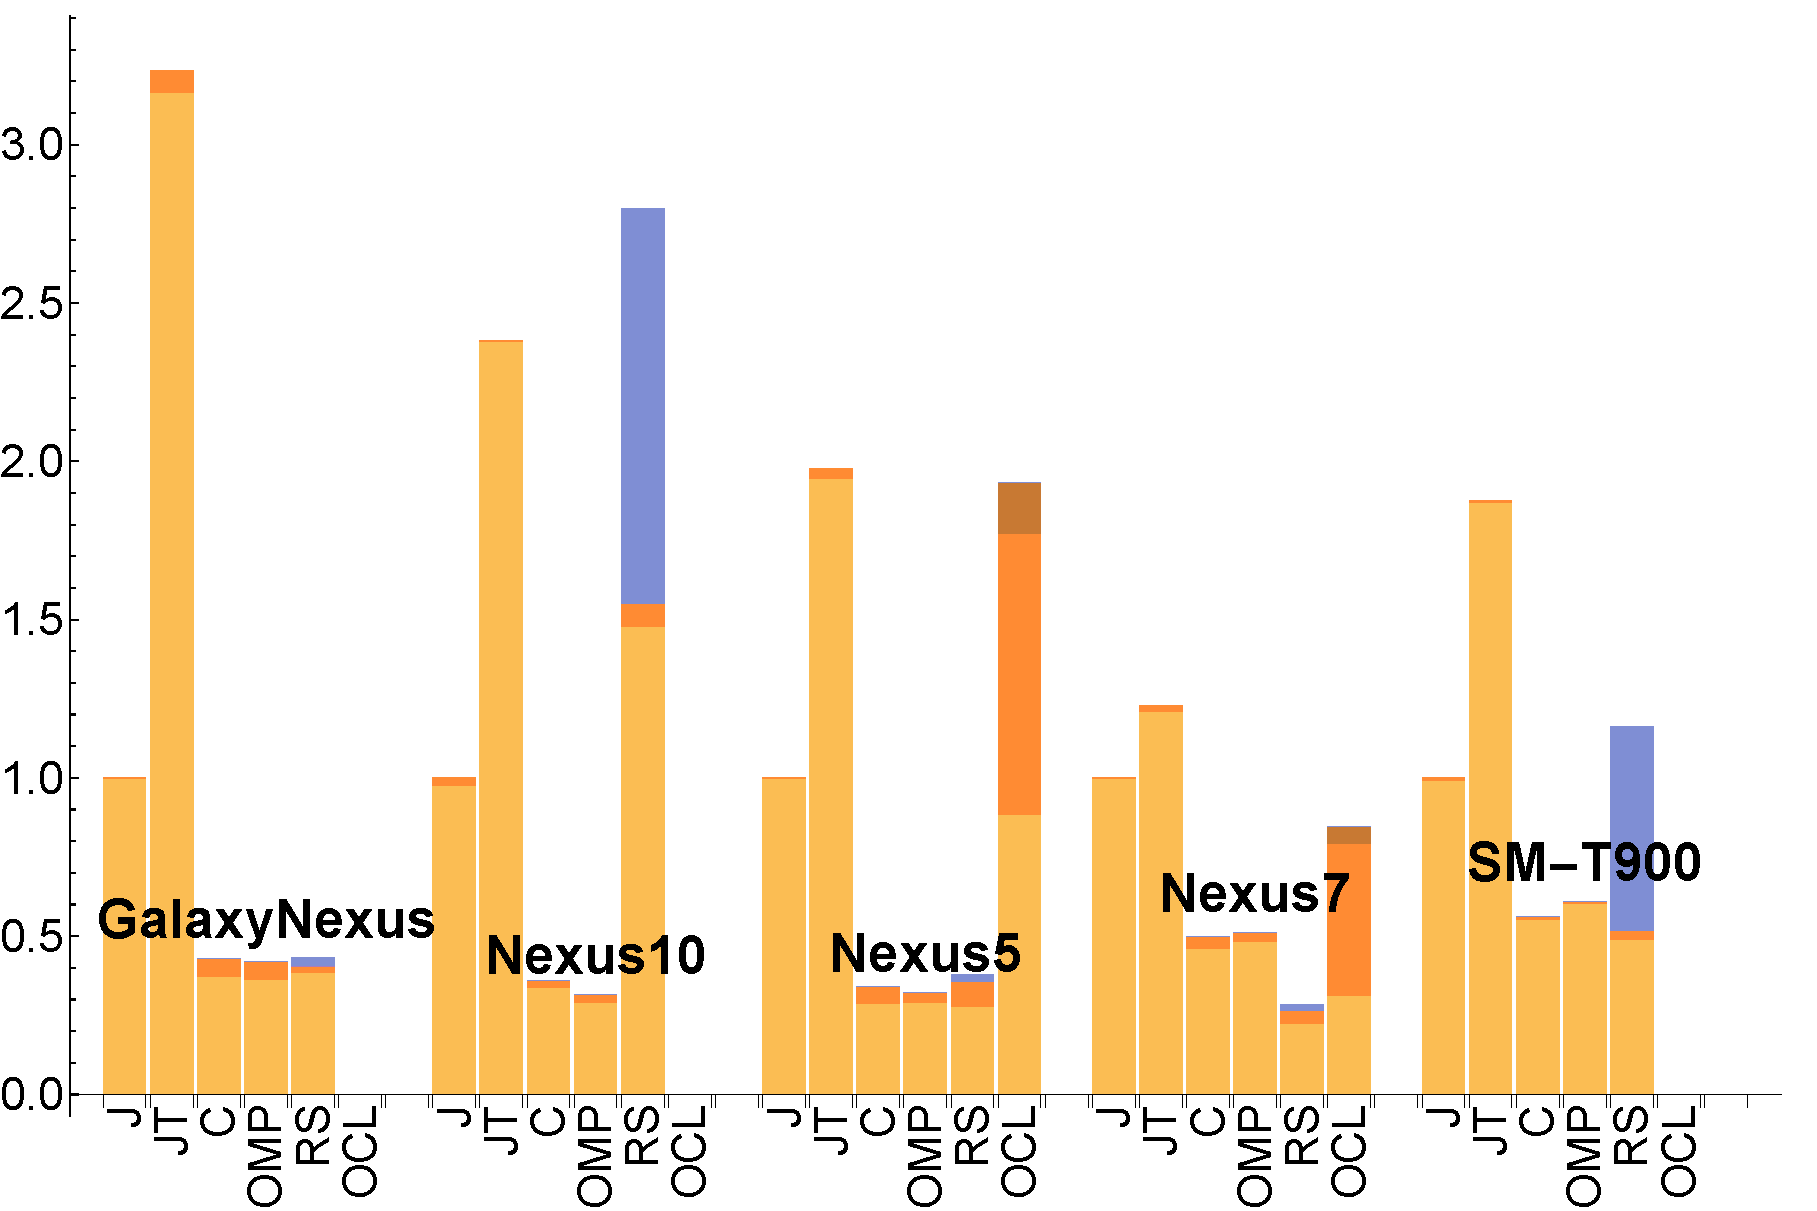
\includegraphics[width=0.9\textwidth]{data/VectorAdd_time.pdf}
      \caption{VectorAdd}
  \end{subfigure}
  \begin{subfigure}[b]{0.33\textwidth}
      \centering
      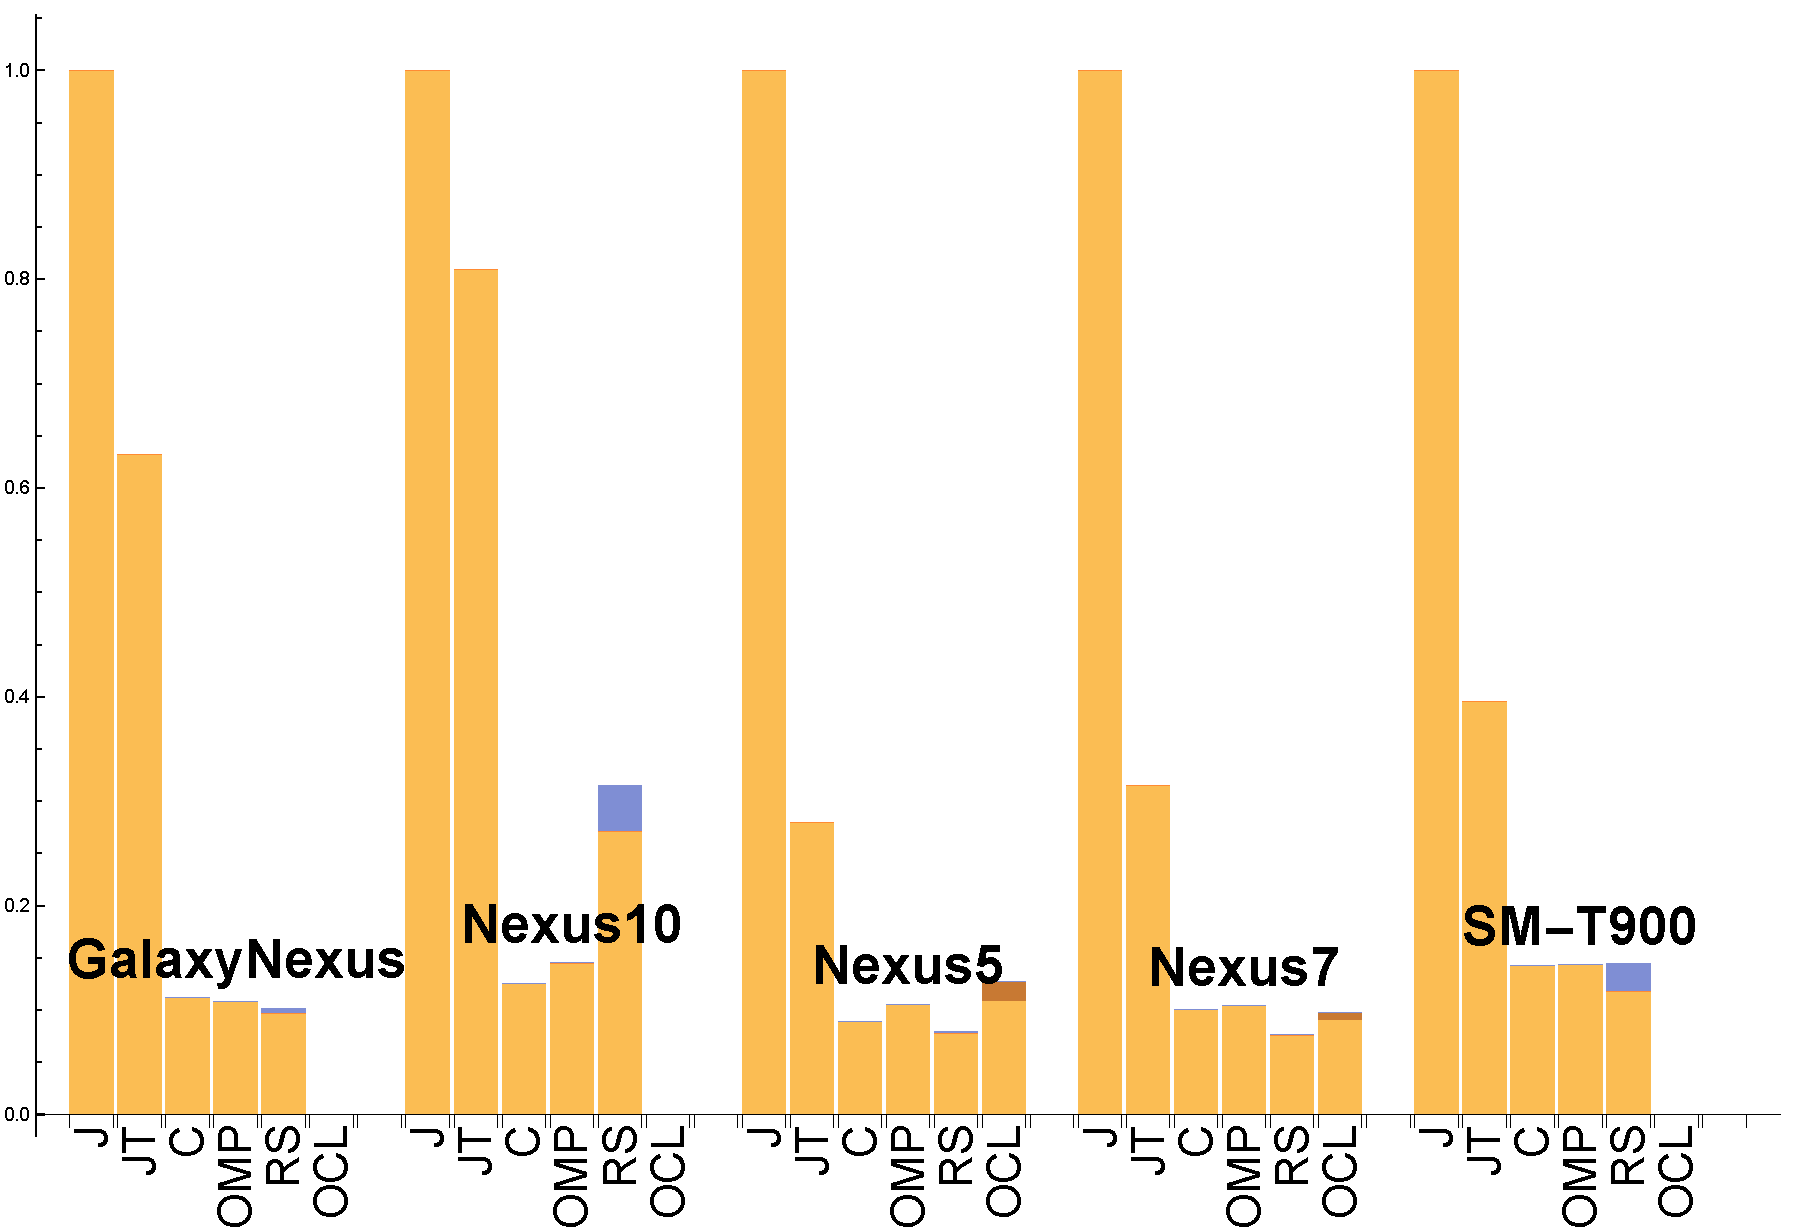
\includegraphics[width=0.9\textwidth]{data/Sgemm_time.pdf}
      \caption{Sgemm}
  \end{subfigure}
  \begin{subfigure}[b]{0.33\textwidth}
      \centering
      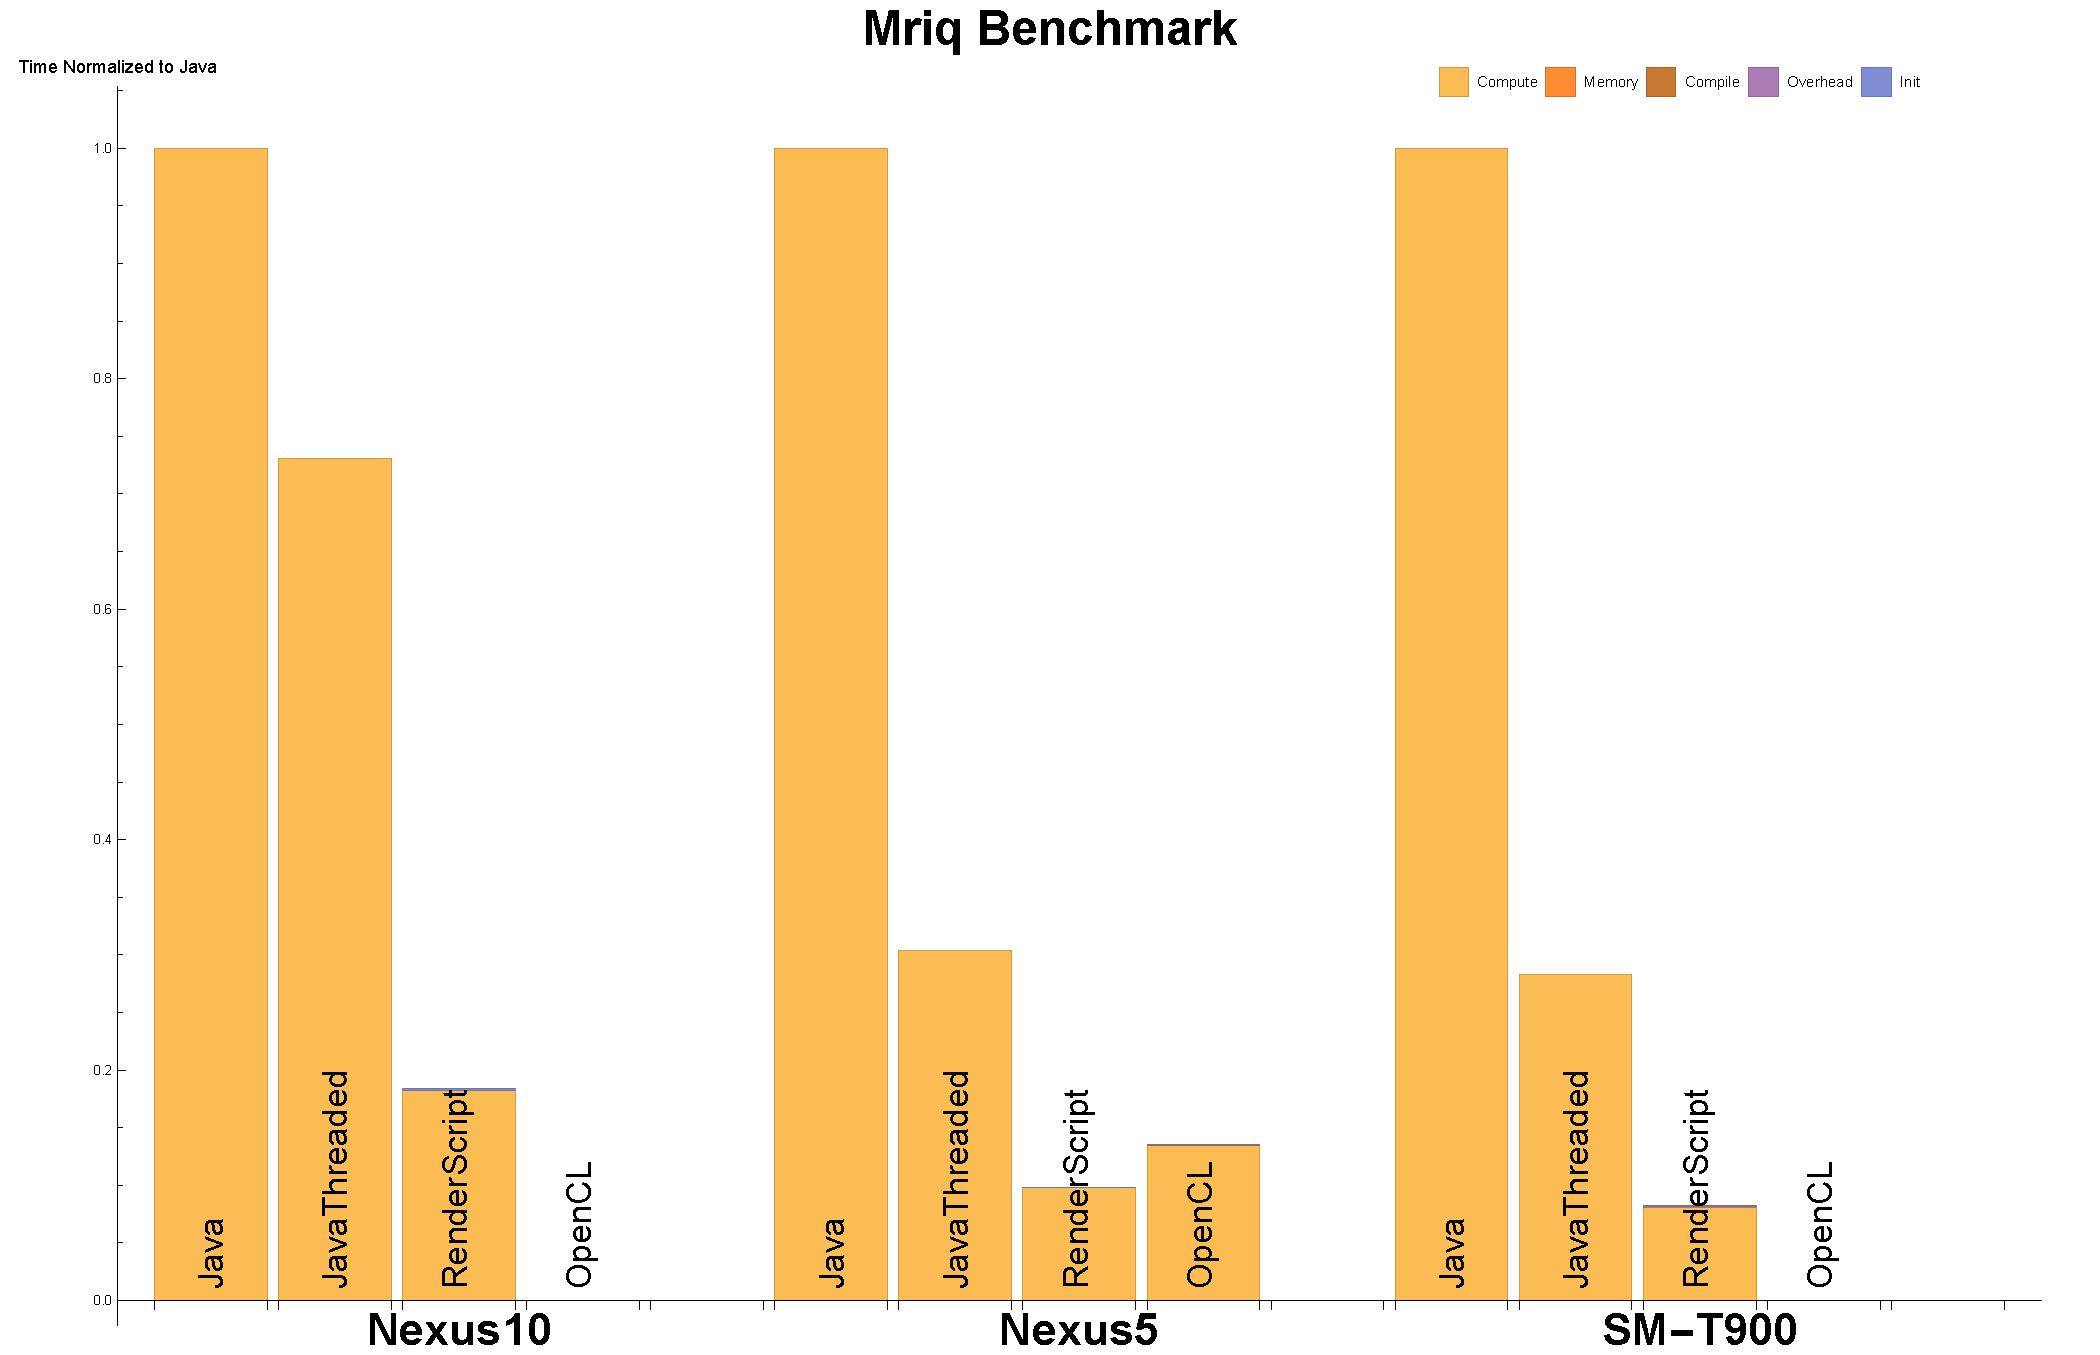
\includegraphics[width=0.9\textwidth]{data/Mriq_time.pdf}
      \caption{MRIQ}
  \end{subfigure}

  \begin{subfigure}[b]{0.33\textwidth}
      \centering
      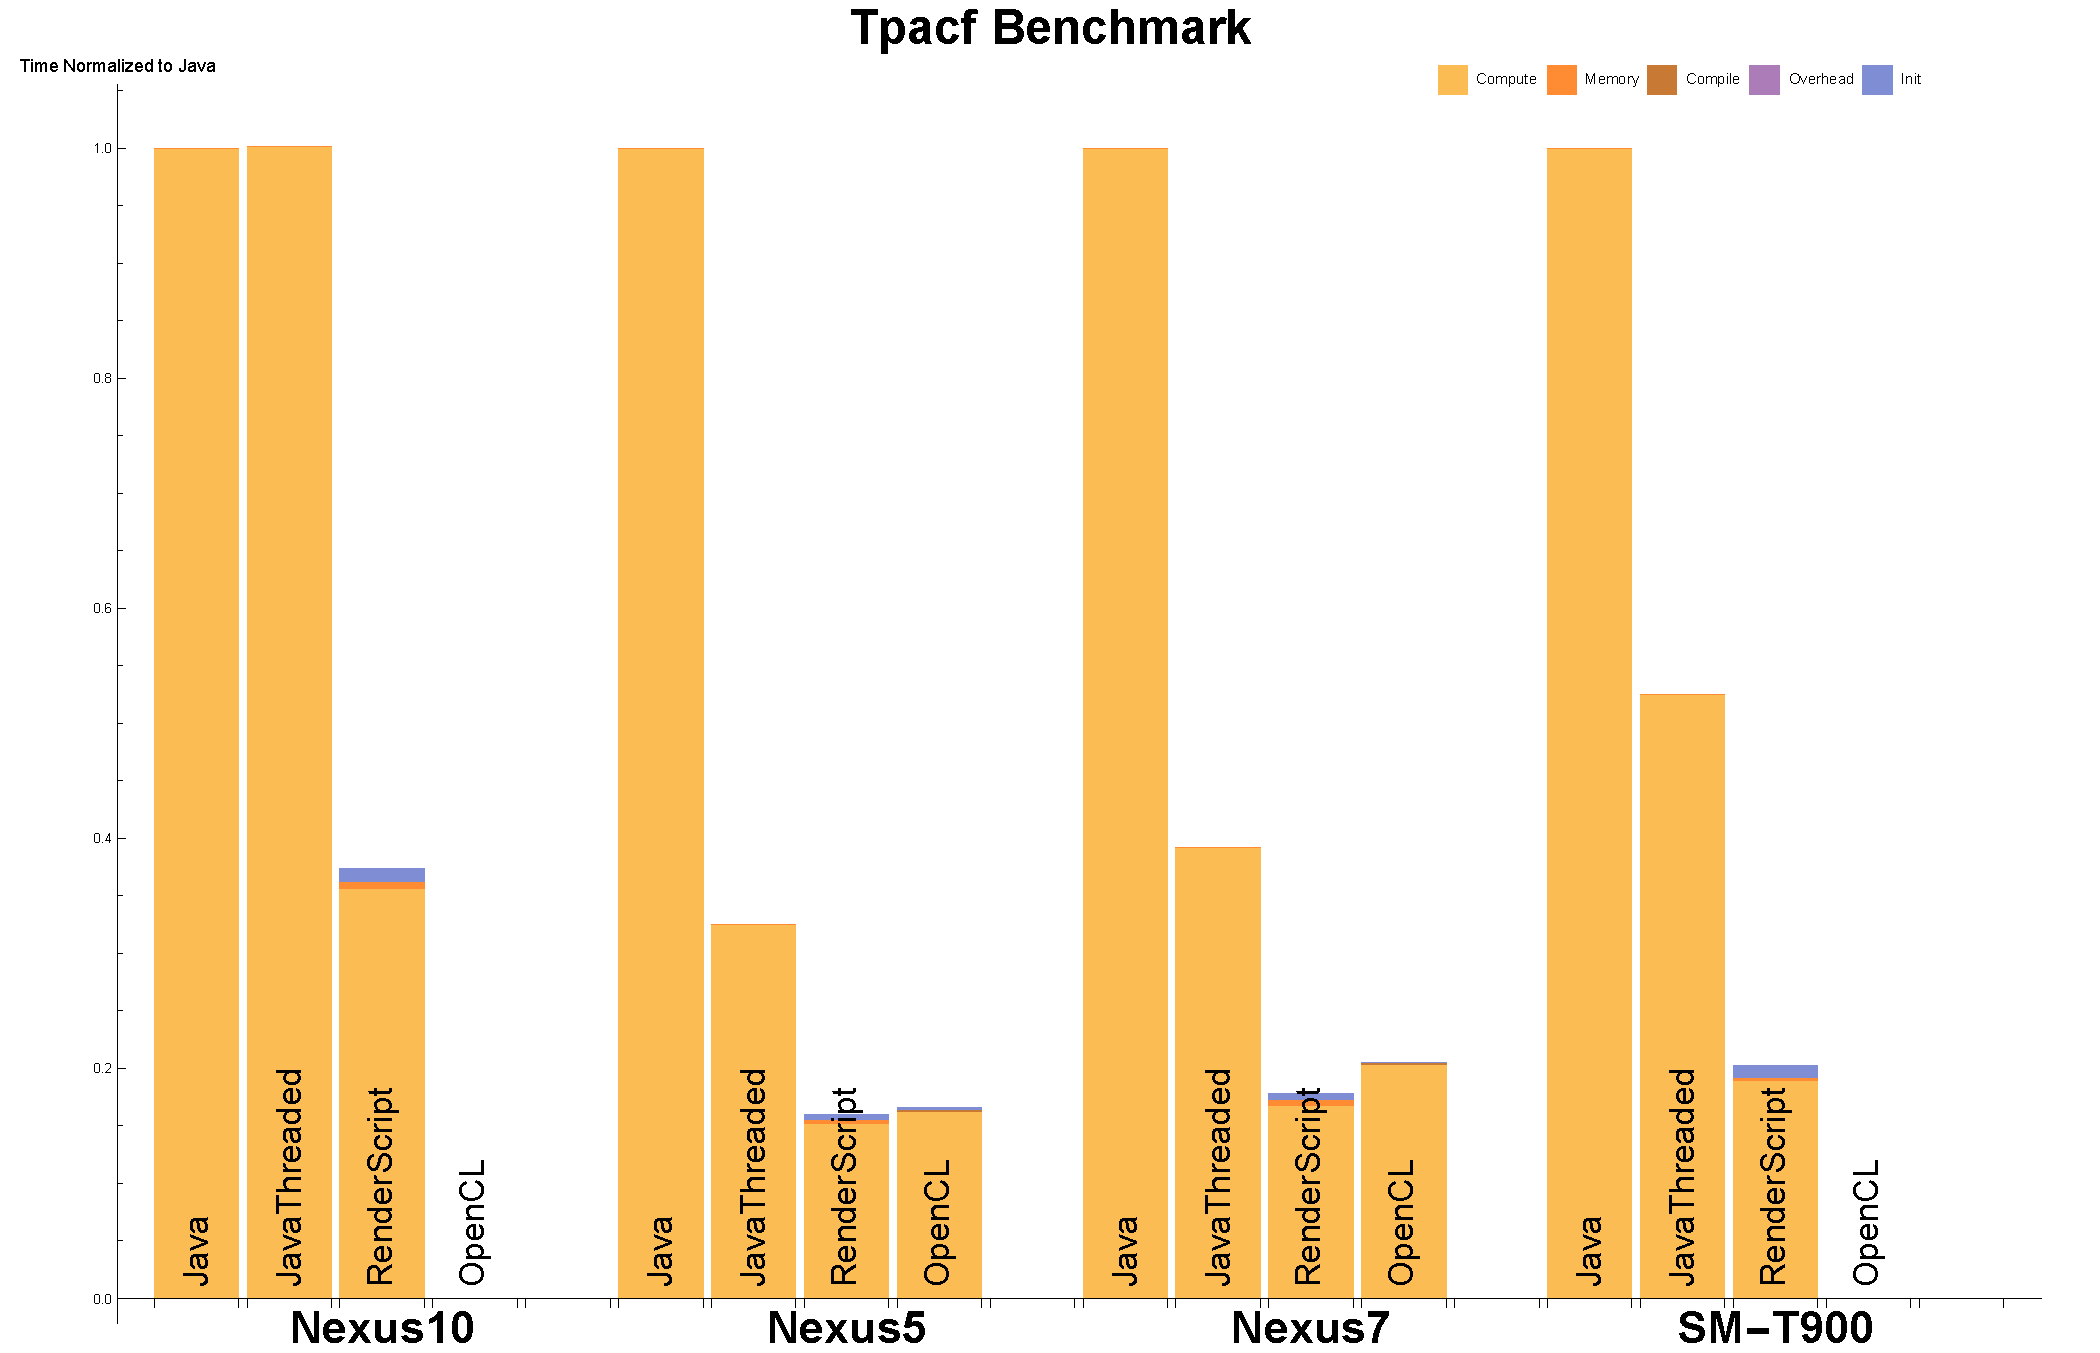
\includegraphics[width=0.9\textwidth]{data/Tpacf_time.pdf}
      \caption{TPACF}
  \end{subfigure}
  \begin{subfigure}[b]{0.33\textwidth}
      \centering
      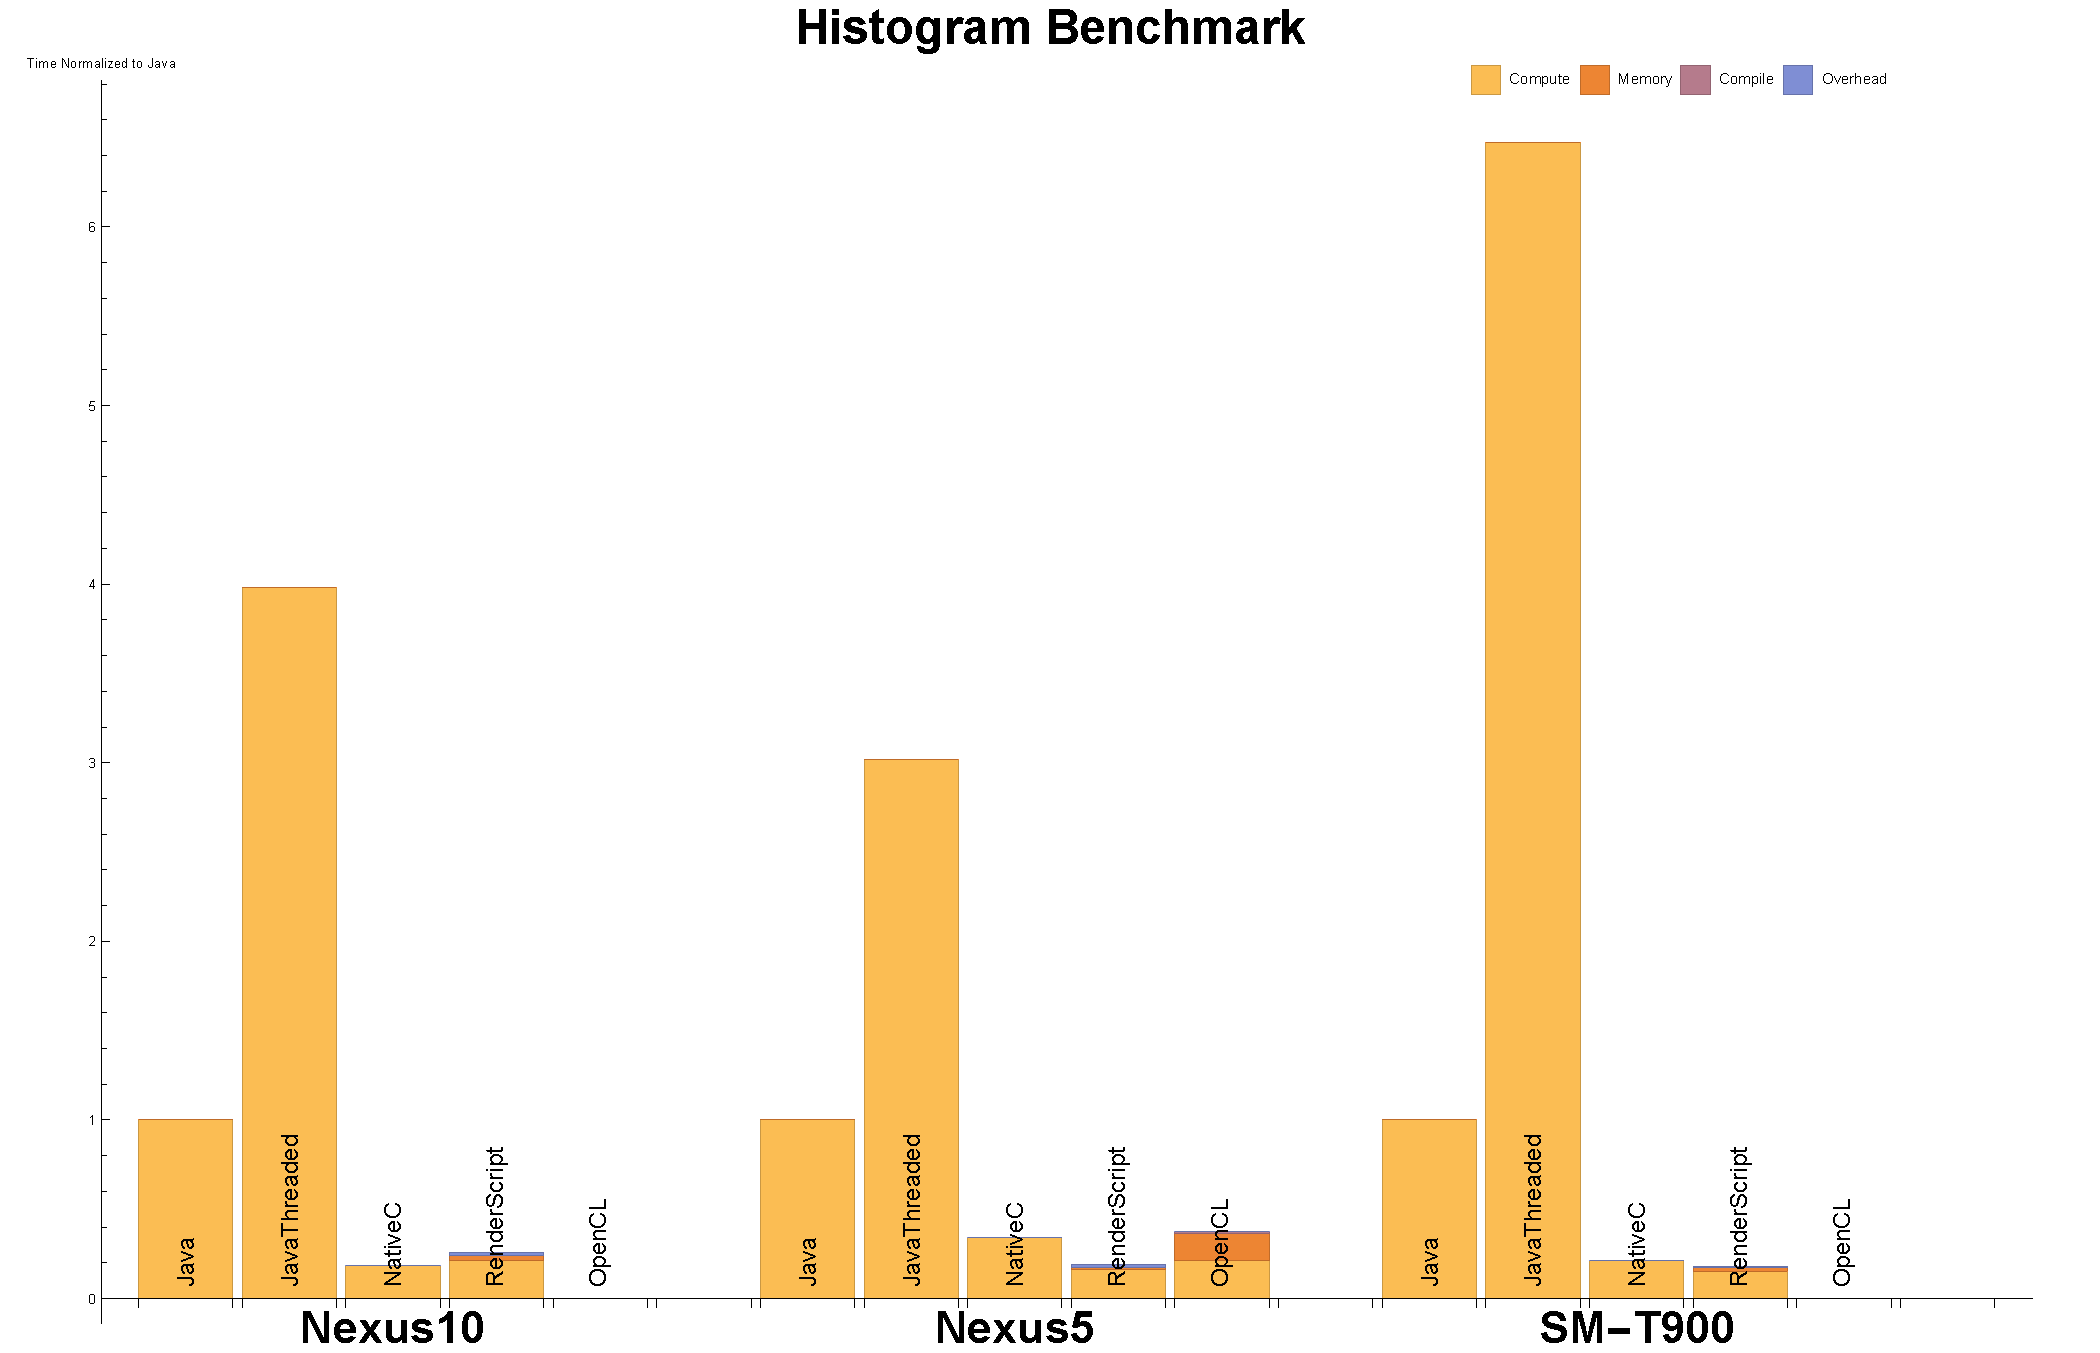
\includegraphics[width=0.9\textwidth]{data/Histogram_time.pdf}
      \caption{Histogram}
  \end{subfigure}
  \begin{subfigure}[b]{0.33\textwidth}
      \centering
      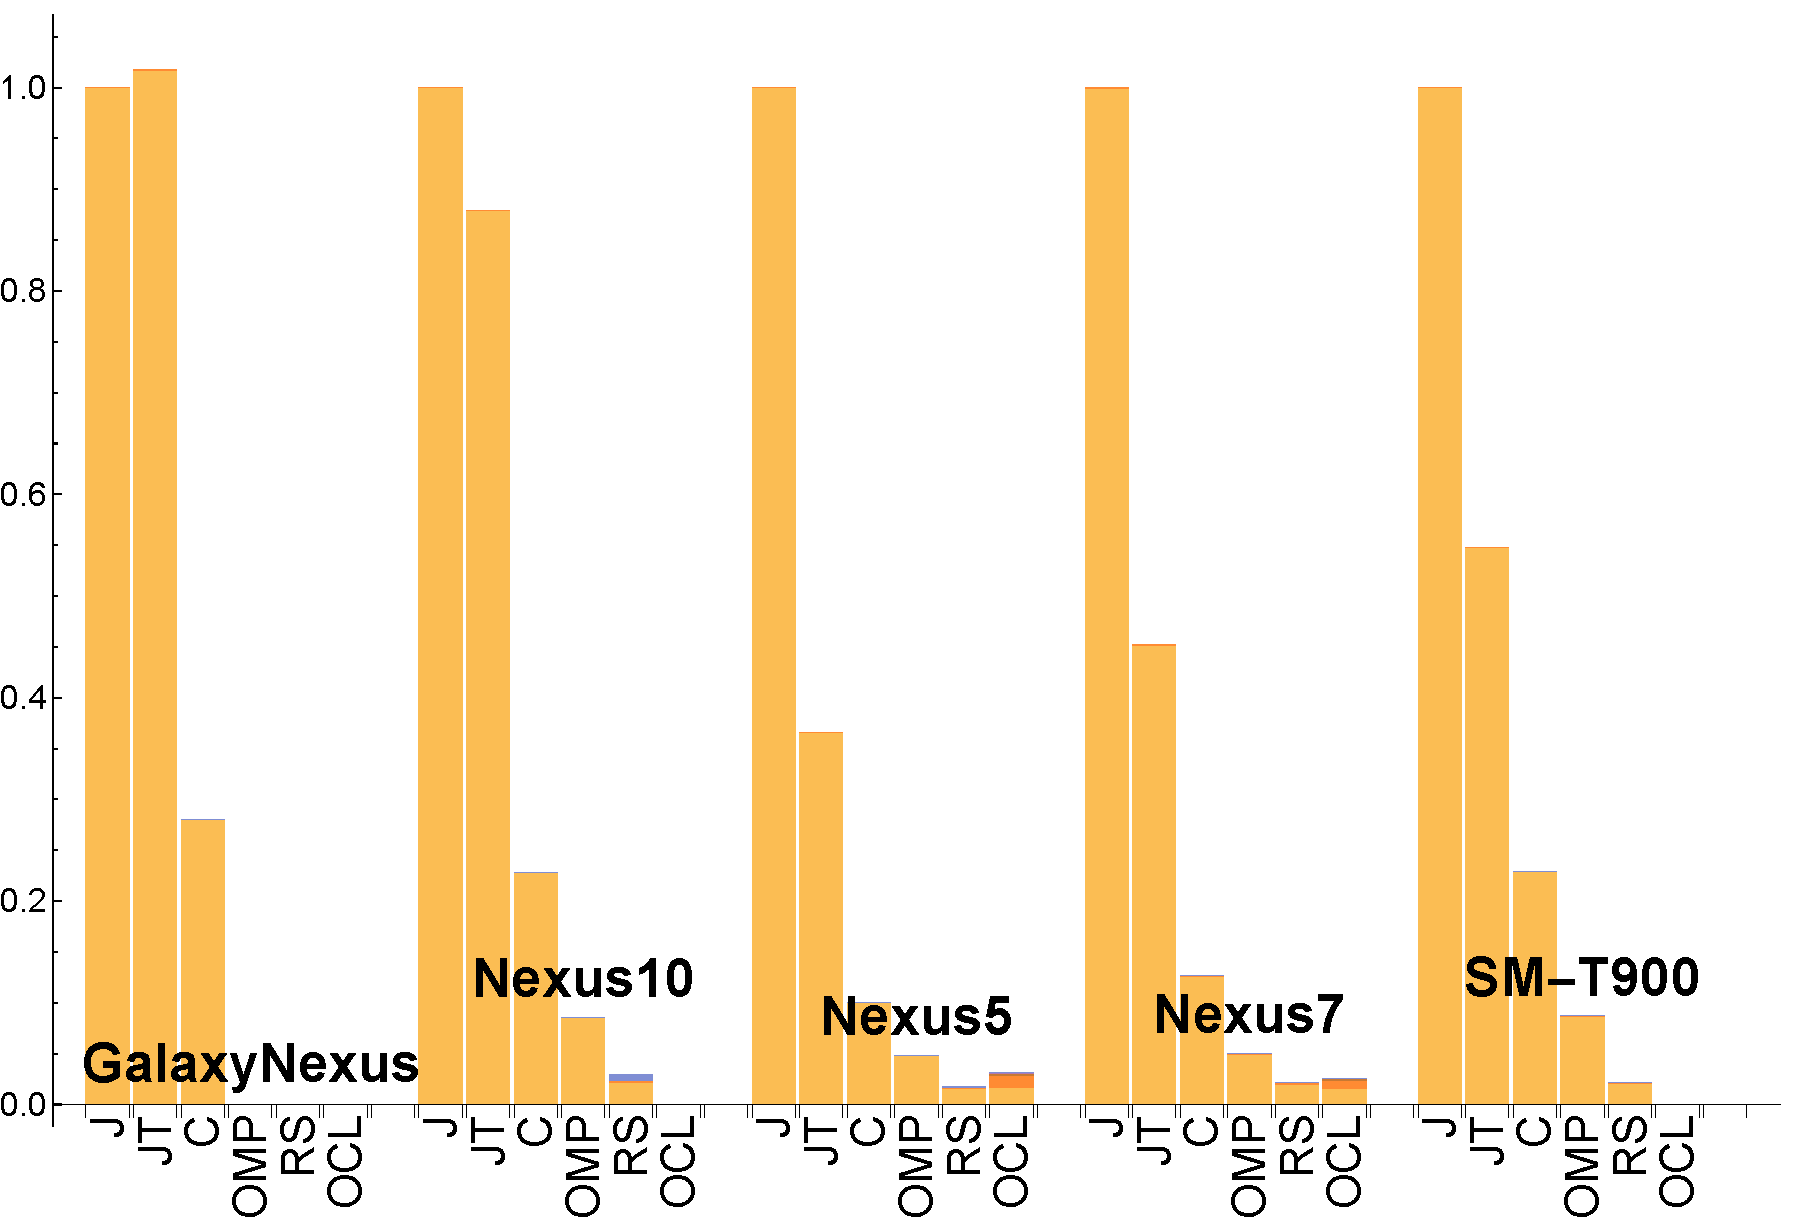
\includegraphics[width=0.9\textwidth]{data/Stencil_time.pdf}
      \caption{Stencil}
  \end{subfigure}

  \caption{Runtime across devices where kernel is executed multiple times. The runtime is normalized to the Java execution time (lower is better). J : Java, JT : JavaThreaded, C : Native C, OMP: OpenMP, OCL : OpenCL, and RS : RenderScript.}
  \label{fig:perfMany}
\end{figure*}


Performance is measured by timing code within regions of code while the device is plugged into the development machine.
Each compute part of an implementation is run $5$ times with the minimum
  presented.
We consider two cases --- one where the kernel code is run once (figure~\ref{fig:perfOne}) and therefore
  the overhead (memory, compilation, and initialization) has a big impact on perfomance,
  and one where the kernel is run $100$ times (figure~\ref{fig:perfMany}) (or $5$ for both TPACF and MRIQ)
  and the overhead has little impact.

For each device, the plot show the time taken to execute sections of the code normalized
  to the Java execution time.
These times correspond to the $x$-axis of the processor utilization times discussed
  in the previous section (e.g. figure~\ref{fig:loadVecAddSgemm}) --- Trepn is not
  running while collecting these timing results.
Not all benchmarks were run on the GalaxyNexus, since the device,
  being low end, takes a long time to execute the benchmarks.

In figure~\ref{fig:perfOne} the compute code is only executed once, it is clear that 
  the overhead of RenderScript on the Nexus 10 (and to some extent the SM-T900) device is consistently high.
We suspect that the Nexus 5 and Nexus 7 are using a more recent version of the RenderScript library compared to the Nexus 10.
As one would expect, when a kernel is executed only once, then overhead dominates the time. Thefore, for such executions, it is not a good policy to of-load the computation to either RenderScript or OpenCL ---
  i.e. the programmer still needs to understand which sections of the program are very hot and could benefit by not being hosted 
  in Java.

In figure~\ref{fig:perfMany}, we look at the performance if memory management is optimized and the kernel code is executed 
  many times.
Code with a high memory to compute ratio, such as VectorAdd (and SGEMM to some extent), do not perform well using either
  RenderScript or OpenCL (this is due to poor occupancy in the OpenCL case).
For code that has irregular accesses or with a low memory to compute ratio, we find that RenderScript's compute time is similar
  to that of OpenCL, but is better when also considering overhead time.
Both RenderScript and OpenCL outperform the OpenMP implementation in all benchmarks.

As expected, SGEMM's OpenMP timing is similar to that of sequential C, confirming our hypothesis that the C compiler was not able
  to interpret the OpenMP pragma.
Because of the privatization, which requires allocation of histogram within each thread, the threaded Java implementation performs poorly and is 
  worse than the serial Java implementation.
Consistently, OpenCL results in better speedups on the Nexus 5 versus the Nexus 7 when compared to the on-board CPU. 

The biggest performance gain comes by not using the JVM, however.
Aside from typical JVM overhead, we notice that these kernels are array access extensive.
Since Java's semantics guarantee array accesses are within bounds, an overhead is incurred for the JVM having to perform implicit checks when arrays are accessed.
Java's floating point semantics also do not match modern hardware (which implement the IEEE 754 standard),
  this introduces more overhead where the JVM needs to perform extra checks and
  convert to Java's IEEE representation.
These overheads do not manifest themselves in our native implementations, and
  also use unsafe casts in both our RenderScript and native code
  to avoid Java performing checks to convert datatypes between Java and RenderScript or Java and native code.

Because of the tooling, however, in many cases 
  writing RenderScript is easier that writing C with JNI bindings.
One does not need to interact with the Java garbage collector, as you do 
  need to when accessing raw Java memory in JNI.
